\documentclass[dwyatte_dissertation.tex]{subfiles} 
\begin{document}

\chapter{Title goes here} % come up with something that is actually like the title of a paper

\section{Introduction}
TODO, pull from proposal and proposal-r1.

\section{Methods}

\subsection{Participants}

% 29 D464D EEG 
% 29 Behavioral only
% ===
% 58 total, 27 female (ages 18-28 mean=21)
A total of 58 students from the University of Colorado Boulder participated in the experiment (ages 18-28 years, mean=21; 31 male, 27 female). EEG was recorded from 29 of the participants while they completed the experiment. The remaining 29 participants completed a solely behavioral experiment without EEG recording. All participants were right-handed and reported normal or corrected-to-normal vision. Participants either received course credit or payment of \$15 per hour as compensation for their participation. Informed consent was obtained from each participant prior to the experiment in accordance with Institutional Review Board policy at the University of Colorado.

\subsection{Stimuli}
Novel ``paper clip'' objects similar to those used in previous studies \cite{BulthoffEdelman92,EdelmanBulthoff92,LogothetisPaulsBulthoffEtAl94,LogothetisPaulsPoggio95,SinhaPoggio96} were created using MATLAB. Eight vertices were placed randomly on the surface of a sphere of unit radius and then joined together with line segments. The last and first vertex were also joined to form a closed loop so that line segment terminations were not a salient feature \cite{BalasSinha09b}. Objects were constrained to exclude extremely acute angles between successive segments (less than 20 degrees) and were approximately rotationally balanced (center of mass within 10\% of the origin). Objects were were rotated completely about their vertical axis in steps of 12 degrees and rendered to bitmap images under an orthographic projection. A total of 16 objects were created using this procedure, yielding 480 images (30 images per object). Object examples are shown in Figure \ref{fig:paperclip}.

% paperclip fig
% rotations for one obj, several objs
\begin{figure}[h!]
\centering
\begin{tabular}{ll}
\textbf{A} \\
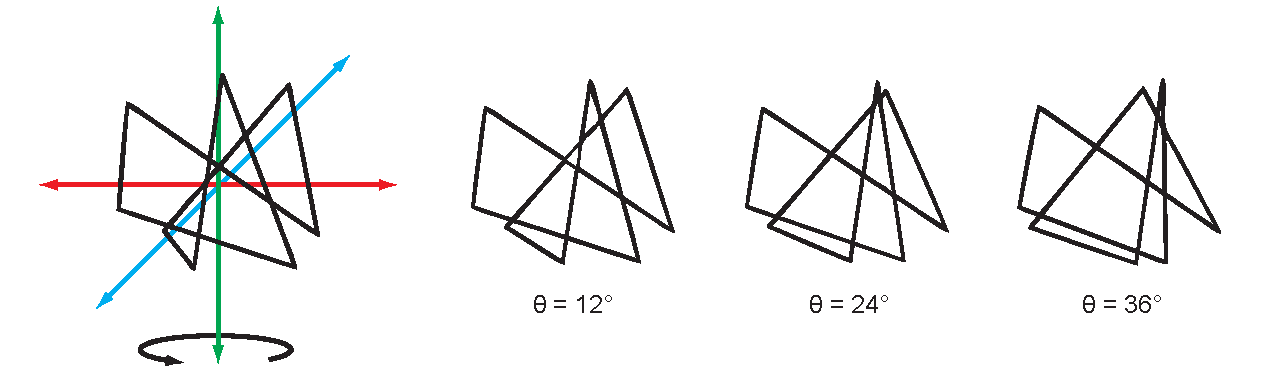
\includegraphics[width=160mm]{figs/pleast/paperclip_rots.pdf} \\
\vspace{5mm} \\
\textbf{B} \\
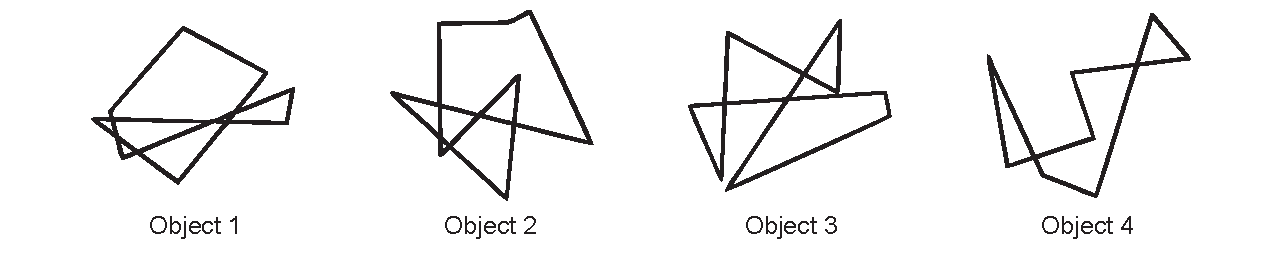
\includegraphics[width=160mm]{figs/pleast/paperclip_objs.pdf} \\
\end{tabular}
\caption{Novel ``paper clip'' objects.}{\textbf{A:} \textbf{B:}}
\label{fig:paperclip}
\end{figure}

\subsection{Procedure}
Participants observed an entraining sequence of rotated views of a random object and performed a same-different judgement about a probe stimulus. On each trial, a view was randomly selected as the initial view of the sequence followed by seven additional views spaced 24 degrees apart (Figure \ref{fig:task}A, blue tick marks). Thus, the eight view entraining sequence spanned 168 degrees of the object. The entraining sequence was either presented in order (i.e., spatially predictable) or randomized. Following the entraining sequence after a 200 ms blank was a probe stimulus consisting of either an unseen view from the entraining object or a novel distractor. Unseen views were randomly sampled from the 12 degree interpolations between views of the entraining sequence (Figure \ref{fig:task}A, magenta tick marks) and from outside of the span of the entraining sequence in increments of 24 degrees (Figure \ref{fig:task}A, green tick marks).

Distractors were created from the original target objects by randomly selecting new spherical coordinates for six of the eight vertices and re-rendering them to bitmap images using the same method as the original target objects (12 degree steps about the vertical axis). Distractors conformed to the same constraints as the original target objects (no extremely acute angles, approximately rotationally balanced). Participants were instructed to respond ``same'' if they believed the probe depicted the same object as the entraining sequence or ``different'' if it depicted a distractor object. Participants received feedback after each trial according to whether their response was correct or incorrect. % Responses were collected via a millisecond-accurate response box connected through the display computer's serial port. 

During the entraining sequence, object views were presented for 50 ms at either 10 Hz (i.e., temporally predictable) or at a variable rate by manipulating the interstimulus interval (ISI) between subsequent views. Temporally predictable ISIs were 50 ms, totaling 350 ms across the entraining sequence. Variable ISIs were selected by randomly generating seven ISIs that also summed to 350 ms (Figure \ref{fig:task}B). ISIs were in the range of 16.67 ms (minimum) to 216.67 ms (maximum) in increments of 16.67 ms. Temporal unpredictability was maximized by generating 400 such ISI sequences, calculating the summed squared error (SSE) across subsequent ISIs in a sequence, and selecting the 100 sequences with the highest SSE for use during the experiment.

% task fig
\begin{figure}[h!]
\centering
\begin{tabular}{ll}
\textbf{A} \\
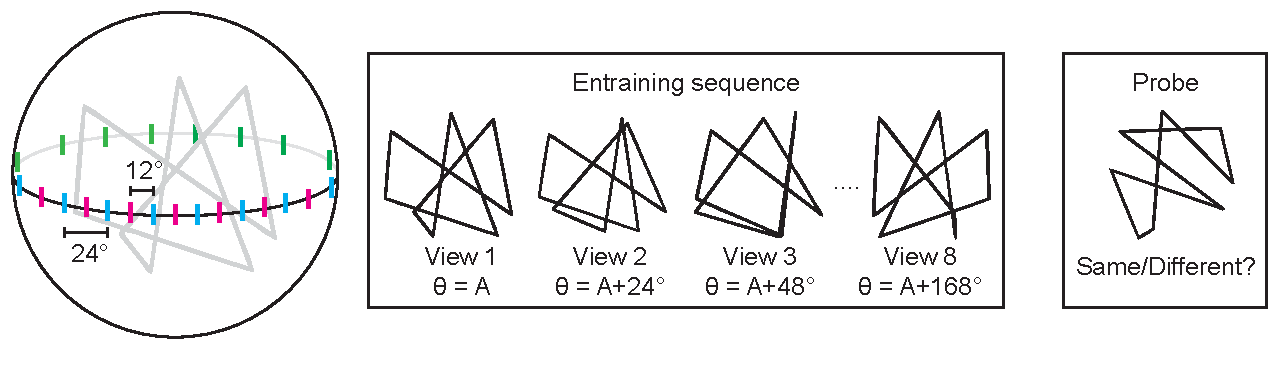
\includegraphics[width=160mm]{figs/pleast/paperclip_task.pdf} \\
\textbf{B} \hspace{90mm} \textbf{C} \\
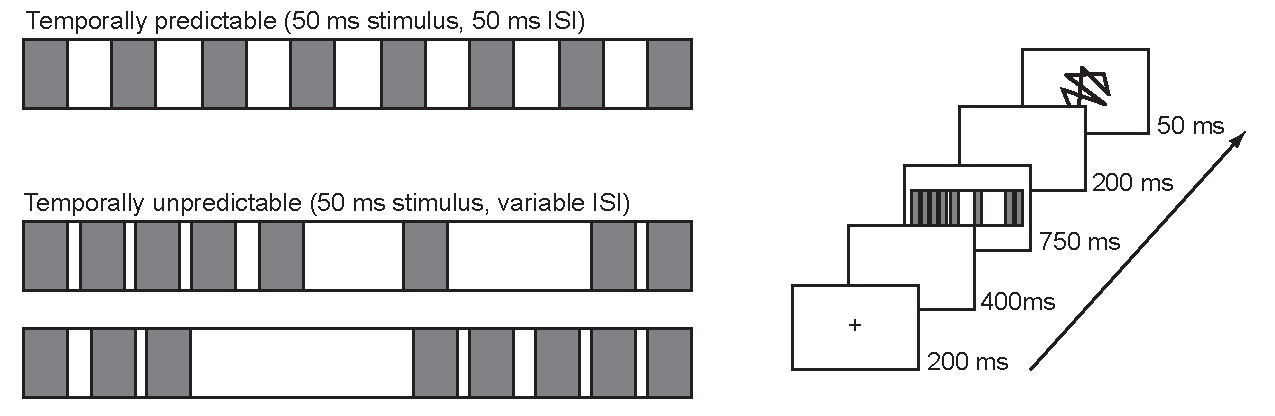
\includegraphics[width=160mm]{figs/pleast/paperclip_ISI.pdf} \\
\end{tabular}
\caption{Experimental procedure.}{\textbf{A:} \textbf{B:} \textbf{C:}}
\label{fig:task}
\end{figure}

The experiment was displayed on an LCD monitor with a native resolution of 1280x1024 operating at 60 Hz using the Psychophysics Toolbox Version 3 \cite{Brainard97,Pelli97}. Stimuli were presented on an isoluminant gray background and subtended approximately 5 degrees of visual angle. Trials began with a fixation cross (200 ms) followed by a blank (400 ms), the entraining sequence (750 ms total), a second blank (200 ms), and ended with the probe stimulus (50 ms) (Figure \ref{fig:task}C). Participants were required to respond within 2000 ms. Trials were separated by a variable intertrial interval of 2000-2400 ms. The experiment contained 500 trials with an additional 20 practice trials that contained a longer blank (1000 ms) between the entraining sequence and the probe to familiarize subjects with the order of events during trials. Participants completed the 20 practice trials (which were discarded from analysis) prior to performing the 500 experimental trials. % random sampling of all variables with replacement

\subsection{EEG recording and preprocessing}
% Net Station 4.3.1
The EEG was recorded using an Electrical Geodesics, Inc. (EGI) system composed of a 128 channel net (HCGSN 130) amplified through 200 M\SI{}{\ohm} amplifiers (Net Amps 200). The signal was sampled at 250 Hz with impedances for each electrode were adjusted to less than 40 k\SI{}{\ohm} before and during the recording. Stimulus and response trigger onsets were measured via the Psychophysics Toolbox using a high precision realtime clock that was synchronized within 2.5 ms of the EEG system's clock before every trial during the experiment.

EEG data were preprocessed using the FieldTrip toolbox \cite{OostenveldFriesMarisEtAl11}. Raw data were first band-pass filtered between 1 Hz and 100 Hz with a 59-61 Hz band-stop and then epoched into 2350 ms segments that spanned the start of the pre-trial blank to 1000 ms after the probe stimulus. Individual segments were visually inspected and rejected if found to contain muscle artifacts or atypical noise. Bad channels were also identified and temporarily removed from the data before performing ICA decomposition \cite{DelormeMakeig04} to remove of ocular artifacts. Components related to ocular artifacts were identified based on their topographical distribution across electrodes. The data were reconstructed without the ocular components and any bad channels were replaced using spherical spline interpolation \cite{PerrinPernierBertrandEtAl89}. The resulting segments were re-referenced to the average reference.

\subsection{Event-related averaging}
Event-related averaging was performed separately for the entraining sequence, the 200 ms blank between before the probe, and the probe itself. For the entraining sequence, the data were baseline corrected 

% entrainer -- 50 ms before each stim? -- try with 100 too
% pre-probe blank -- pre-trial baseline
% probe -- 200 ms pre-probe blank

% revise this since we don't actually care about hemisphere as a factor 
All event-related averaging was further averaged over pools of seven electrodes centered over locations from the 10-10 system that are commonly associated with perceptual processing \cite[e.g.,]{DohertyRaoMesulamEtAl05,RohenkohlNobre11}. These pools included one midline site (OZ) and three sites over each hemisphere (O1/O2, PO3/PO4, and PO7/PO8) (Figure \ref{fig:channels}).

% baseline descriptions here or inline w/ results since it changes per method?
% multiple comparisons
% windowed analysis for N2 for interaction?

% electrode poolings fig
\begin{figure}[h!]
\centering
\begin{tabular}{ll}
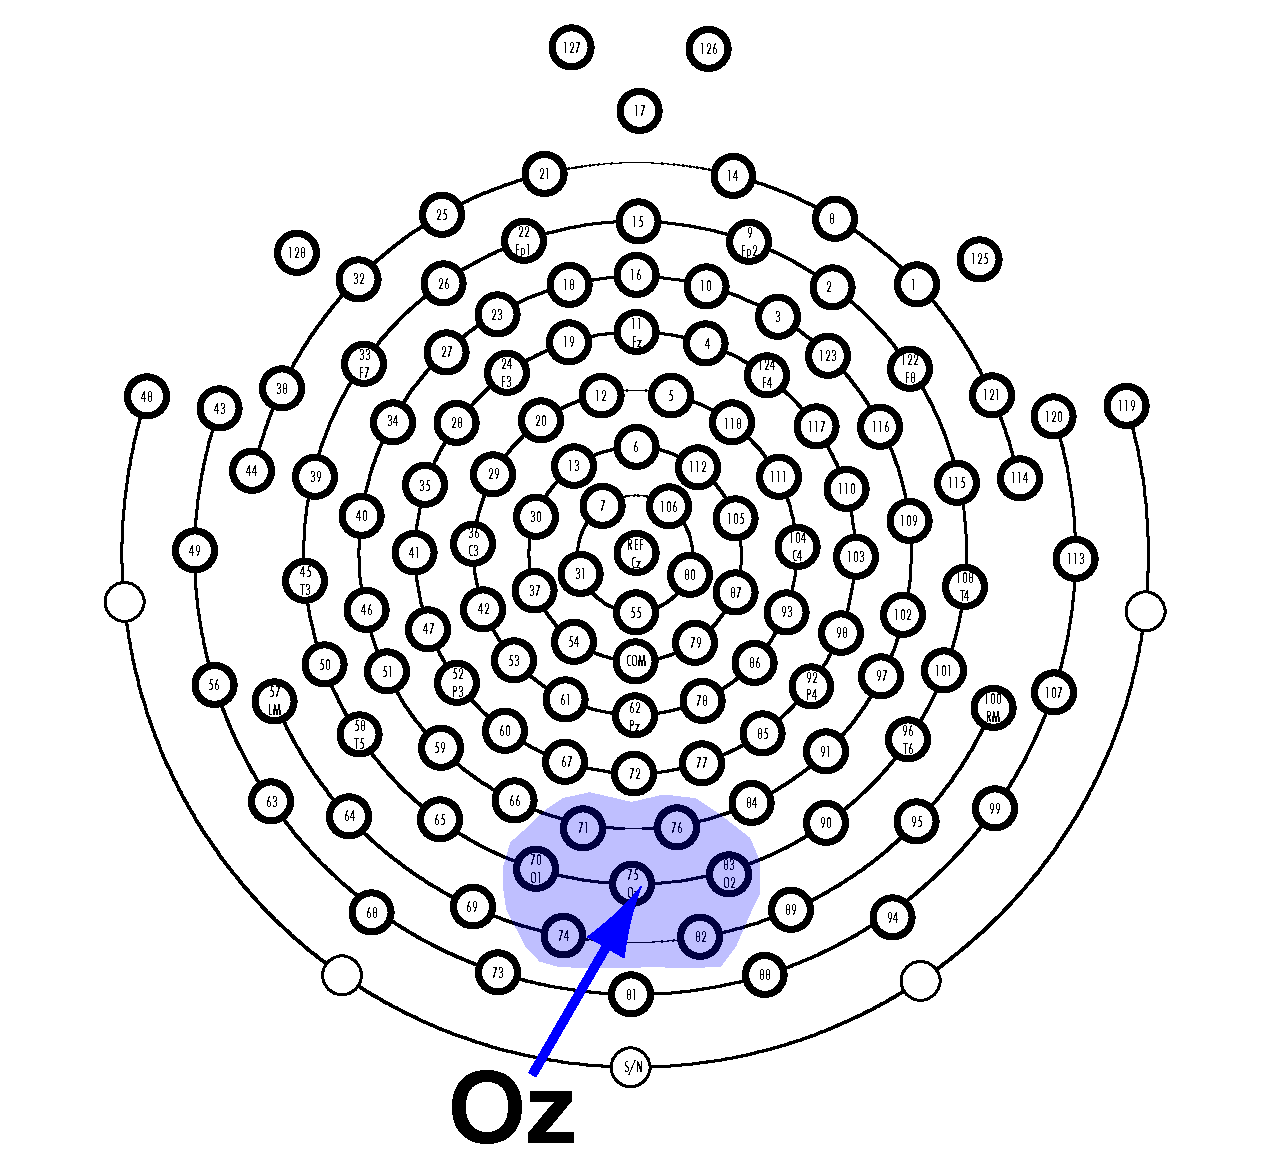
\includegraphics[width=80mm]{figs/pleast/channels_oz.pdf} & 
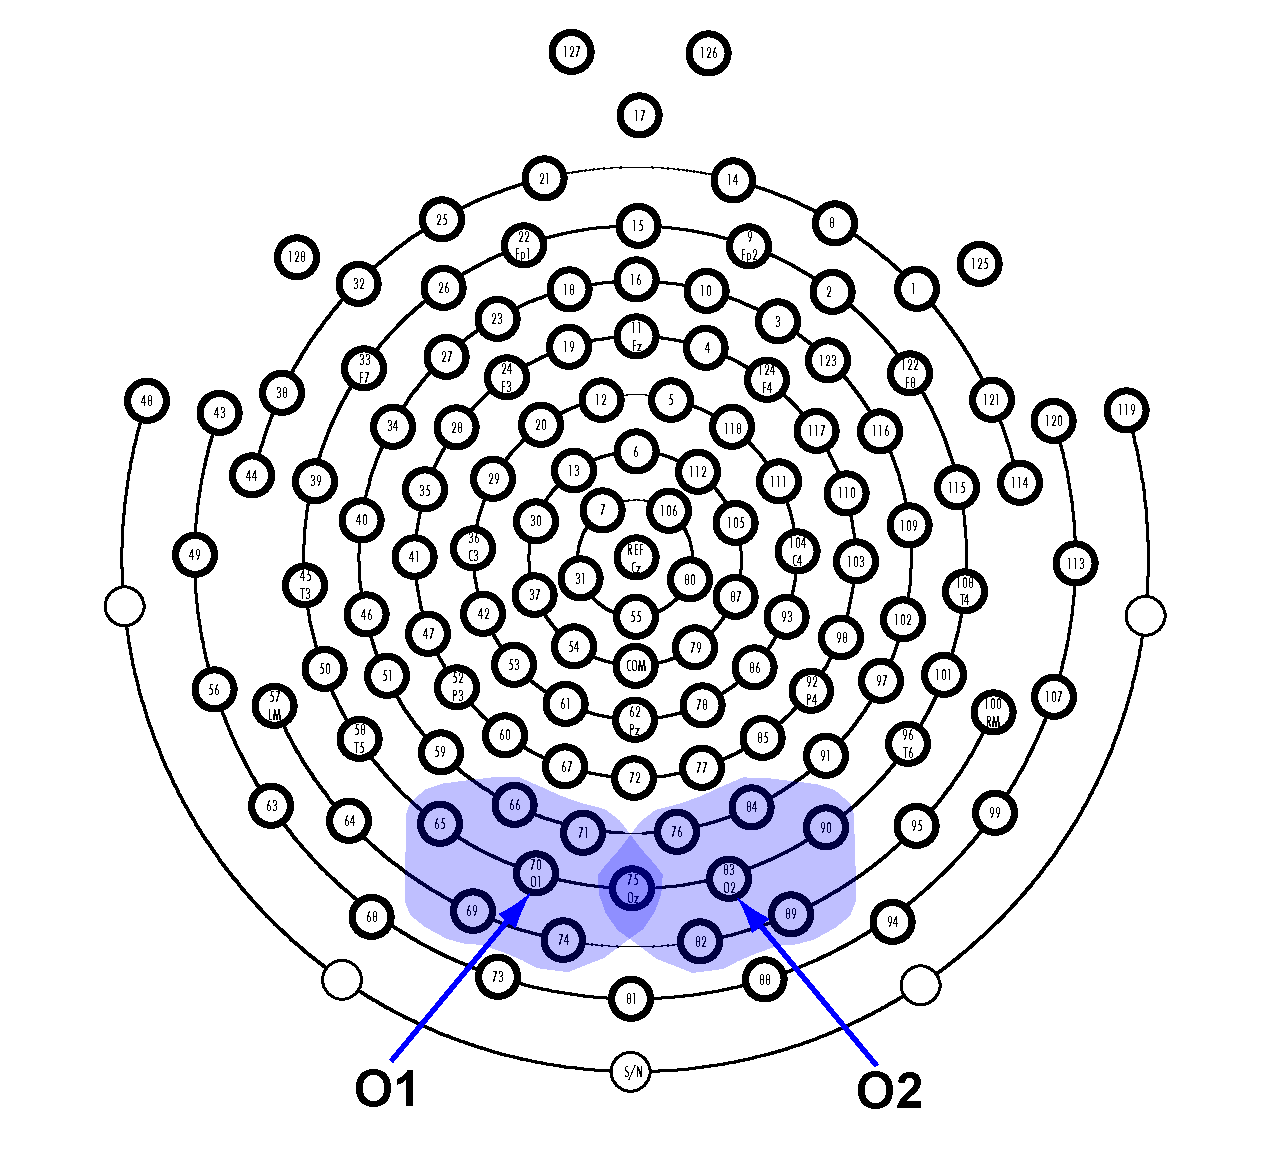
\includegraphics[width=80mm]{figs/pleast/channels_o1_o2.pdf} \\
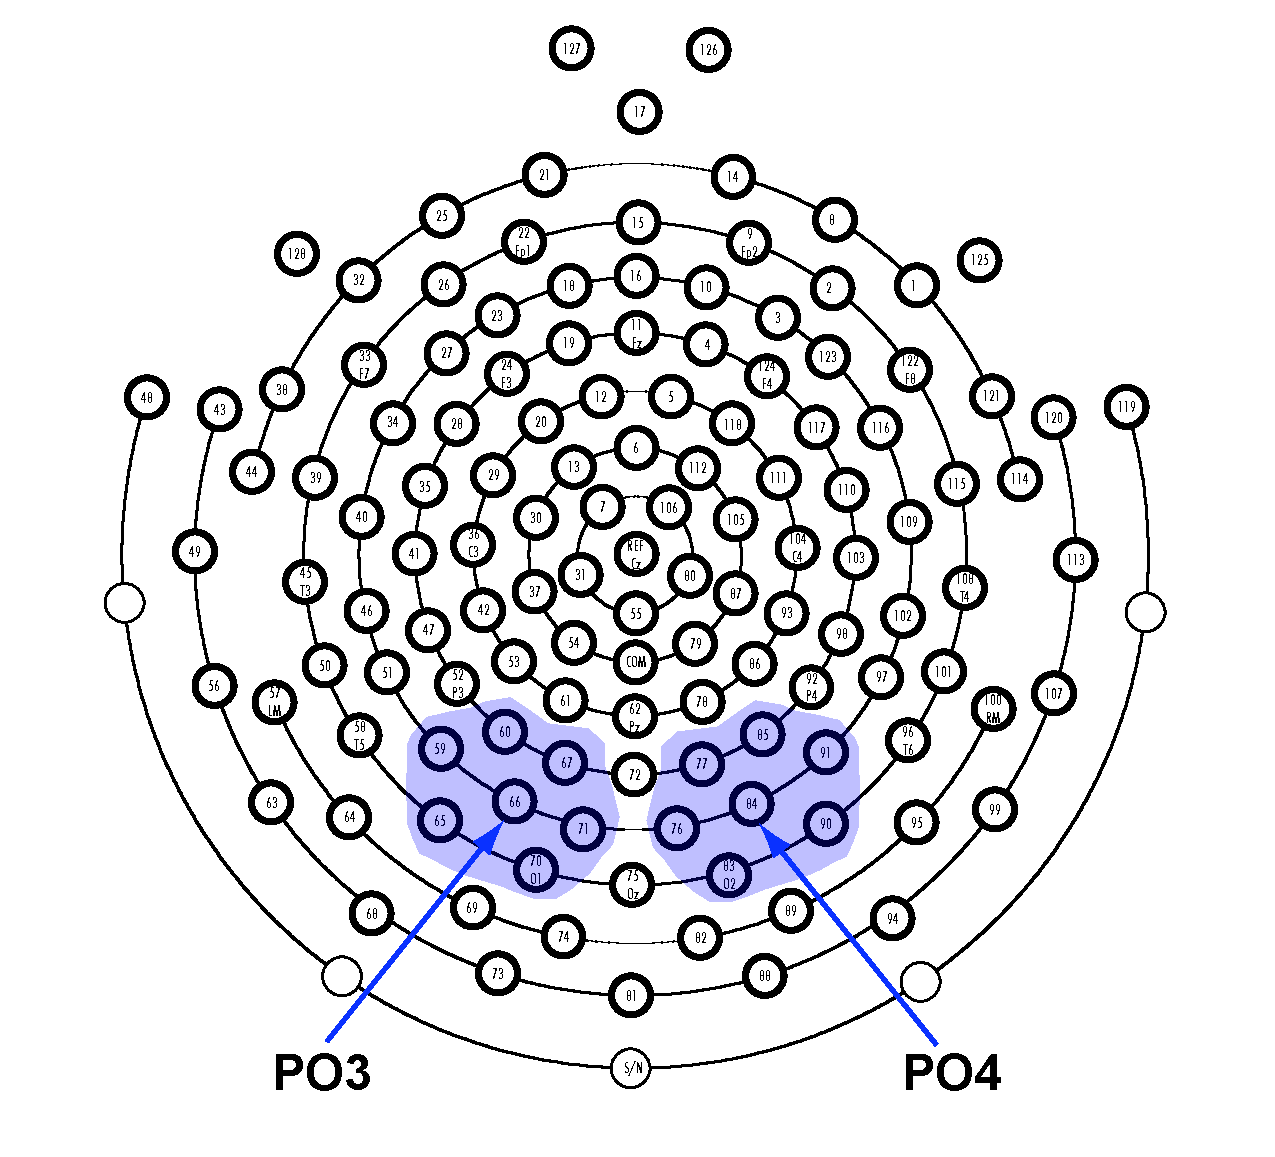
\includegraphics[width=80mm]{figs/pleast/channels_po3_po4.pdf} & 
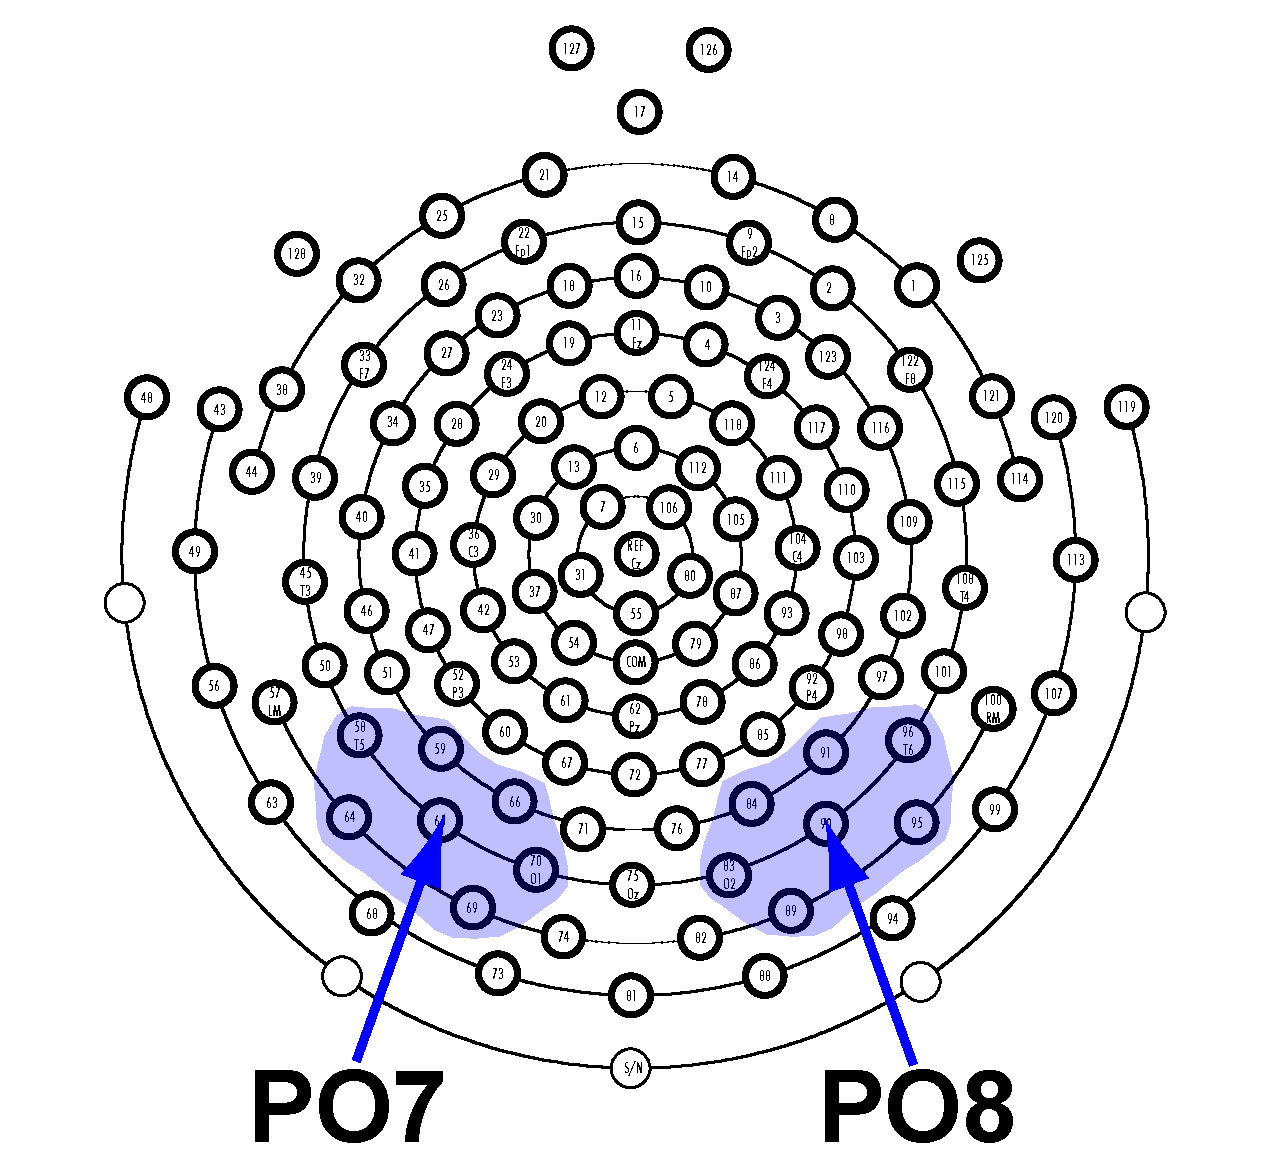
\includegraphics[width=80mm]{figs/pleast/channels_po7_po8.pdf} \\
\end{tabular}
\caption{Electrode poolings.}{}
\label{fig:channels}
\end{figure}

\subsection{Time-frequency analysis}
% convolution method (multitaper)
% equations for ITC/PLV

\begin{align*}
ITC(f,t) = \bigg{|}\frac{1}{N} \sum_{n=1}^{N}{\frac{F_n(f,t)}{|F_n(f,t)|}}\bigg{|}
\end{align*}

\section{Results}

\subsection{Behavioral measures of spatial and temporal predictability}

Five subjects were excluded from behavioral analyses for accuracy 2.7$\sigma$ (or greater) below mean accuracy across subjects. The remaining 53 subjects were submitted to a 2x2 ANOVA with spatial and temporal predictability as within-subjects factors. Experiment type (EEG or behavioral only) was included as an additional between-subjects factor to ensure that it did not interact with any effects.

% acc: spatial F(1,51) = 1.85, p > 0.05
% acc: temporal F(1,51) = 17.84, p < 0.001
% acc: int F(1,51) = 6.13, p = 0.017

% d': spatial F(1,51) = 4.71, p = 0.035
% d': temporal F(1,51) = 11.99, p < 0.001
% d': int F(1,51) = 4.49, p = 0.039

% rt: spatial F(1,51) = 1.957  p > 0.05
% rt: temporal F(1,51) = 12.38, p < 0.001
% rt: int F(1,51) = 0.046, p > 0.05

% ie: spatial F(1,51) = 0.002  p > 0.05
% ie: temporal F(1,51) = 23.31, p < 0.001
% ie: int F(1,51) = 5.849, p = 0.019

% D464B subs acc=75, rt=624.72
% E029 subs acc=0.79 rt=742.1212

% oh, behave
\begin{figure}[h!]
\centering
\begin{tabular}{ll}
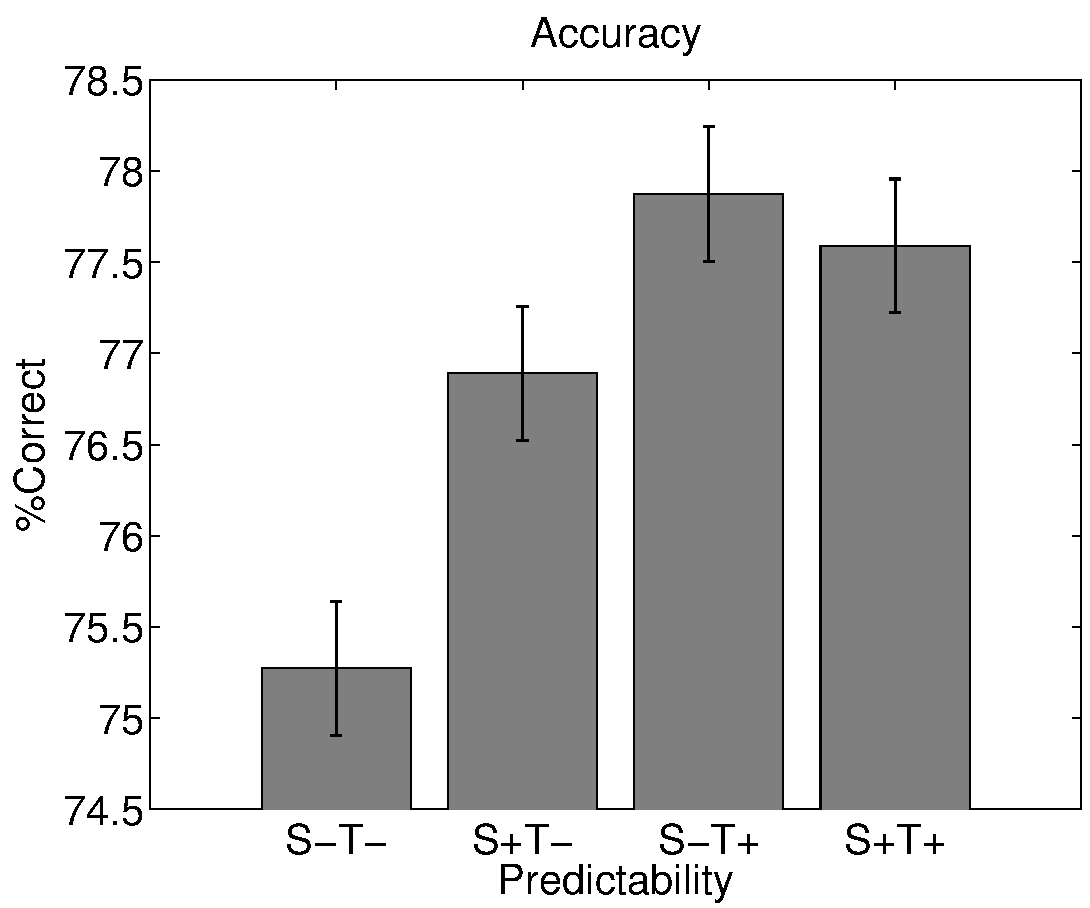
\includegraphics[width=80mm]{figs/pleast/results_accuracy.pdf} & 
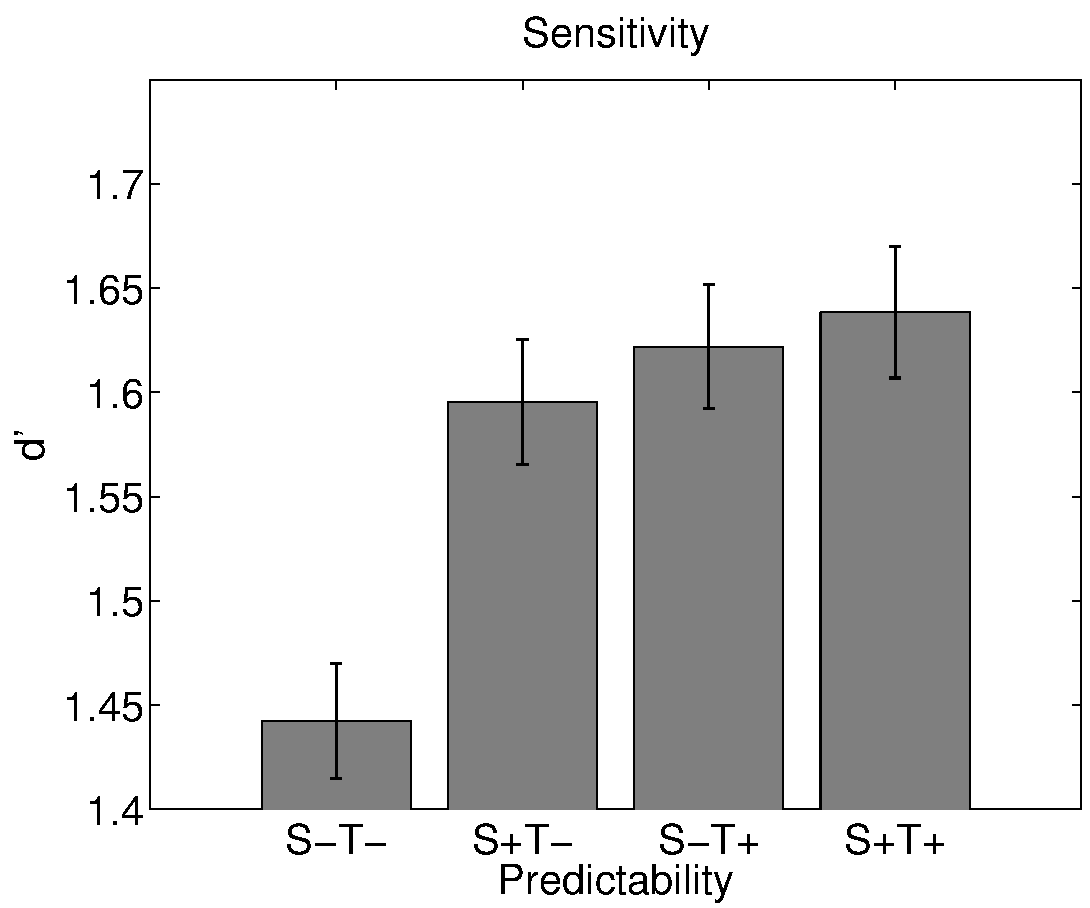
\includegraphics[width=80mm]{figs/pleast/results_dprime.pdf} \\
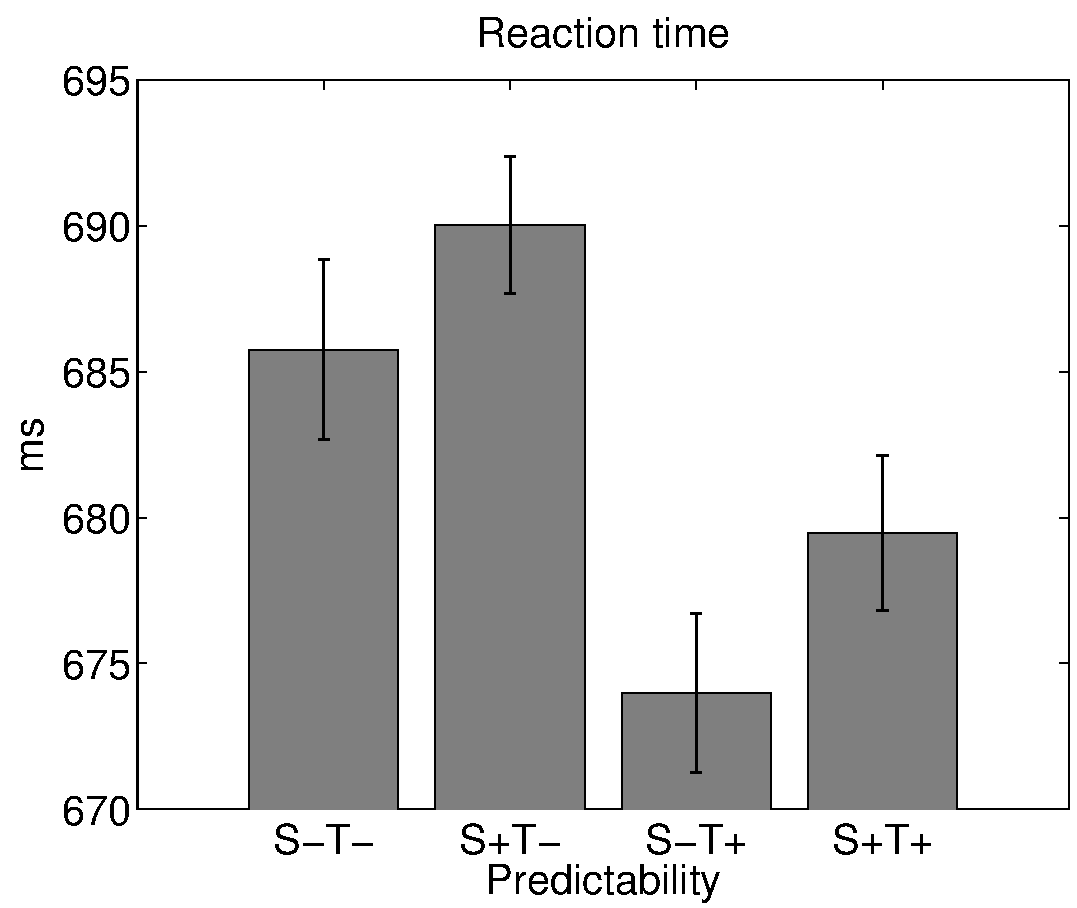
\includegraphics[width=80mm]{figs/pleast/results_rt.pdf} & 
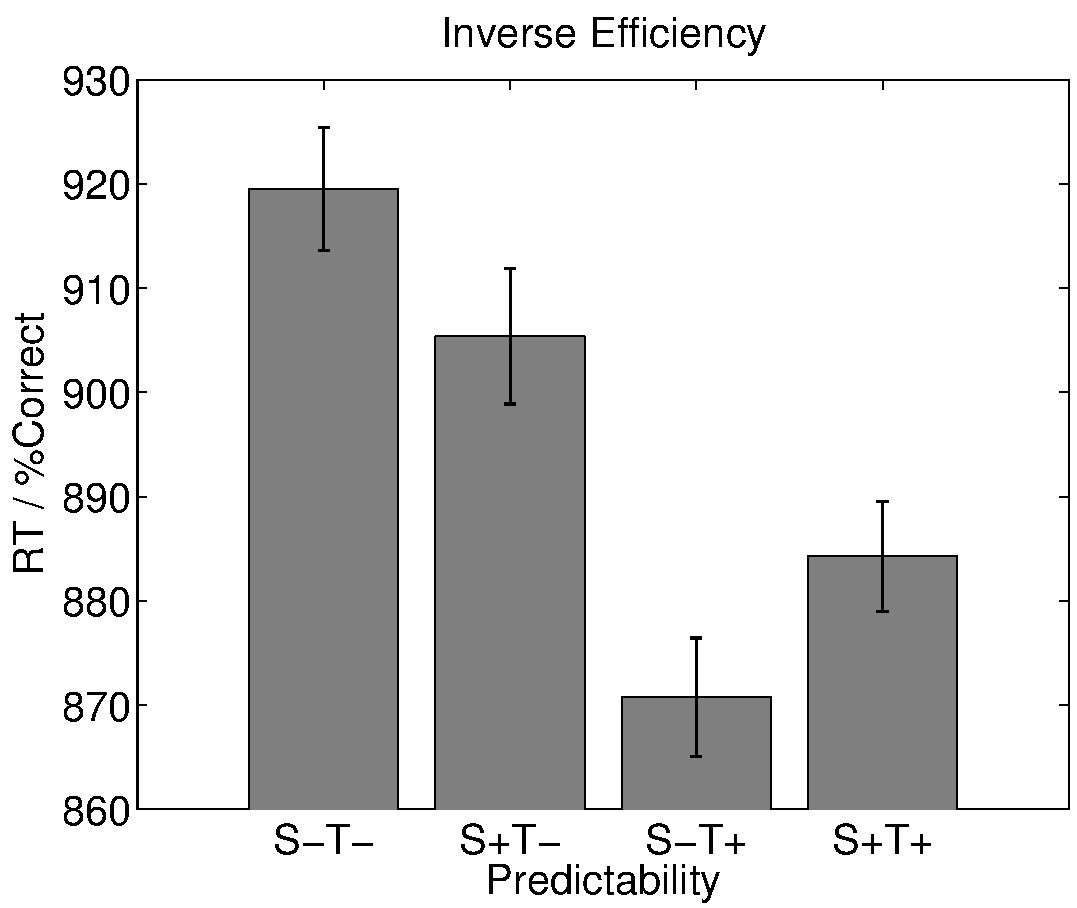
\includegraphics[width=80mm]{figs/pleast/results_ie.pdf} \\
\end{tabular}
\caption{Behavioral measures.}{}
\label{fig:behave}
\end{figure}

% oh, behave pt 2
\begin{figure}[h!]
\centering
\begin{tabular}{ll}
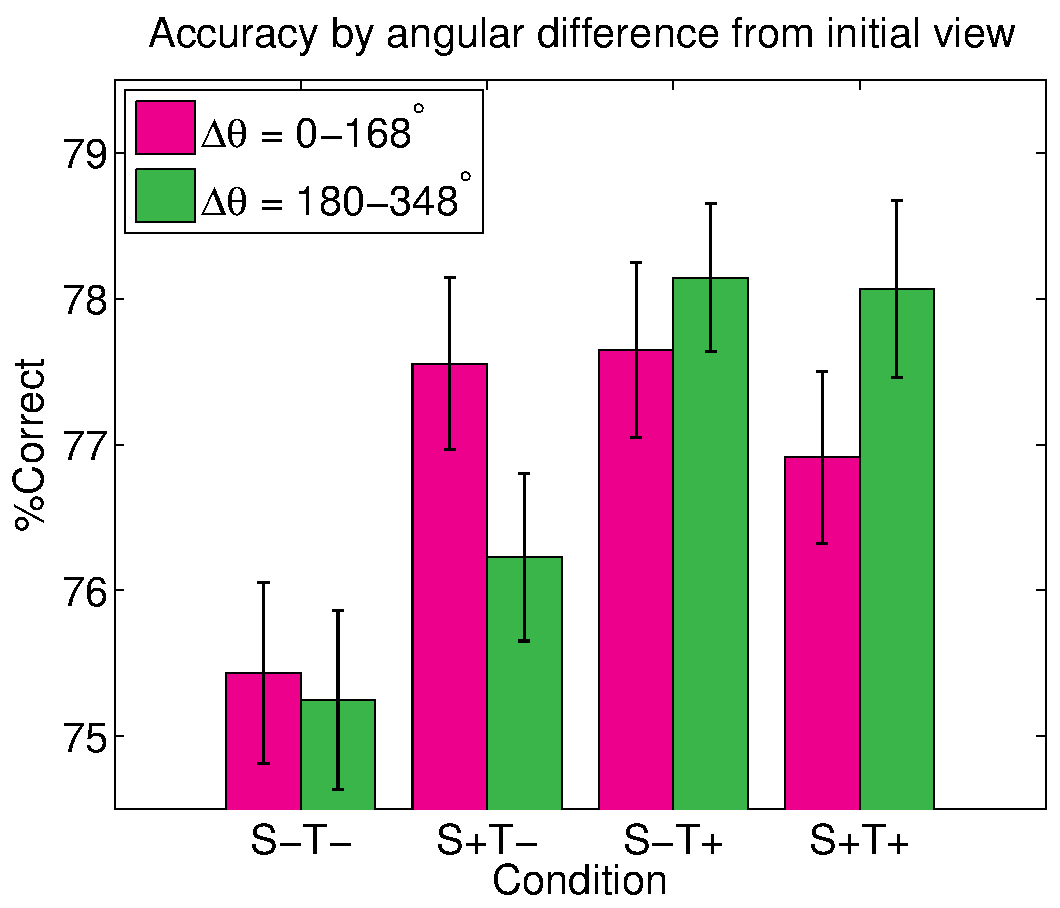
\includegraphics[width=80mm]{figs/pleast/results_accuracy_angle.pdf} & 
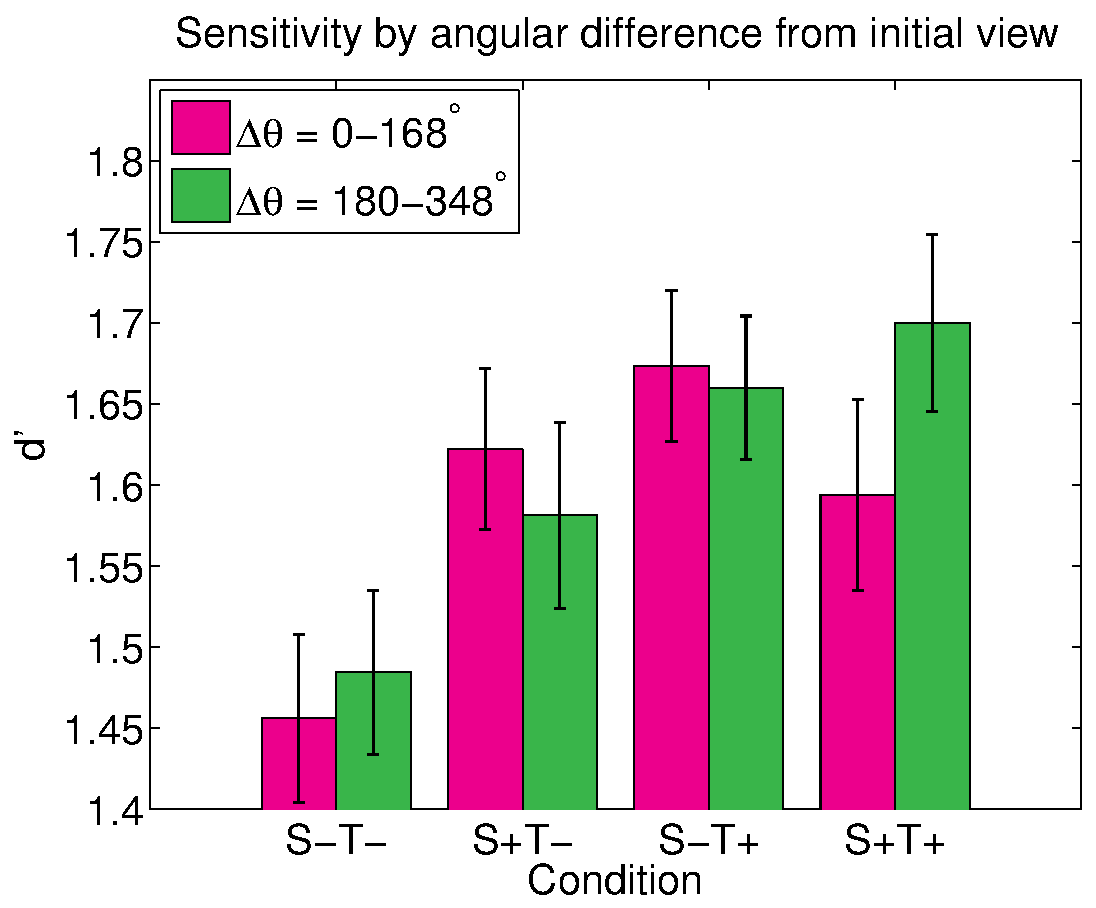
\includegraphics[width=80mm]{figs/pleast/results_dprime_angle.pdf} \\
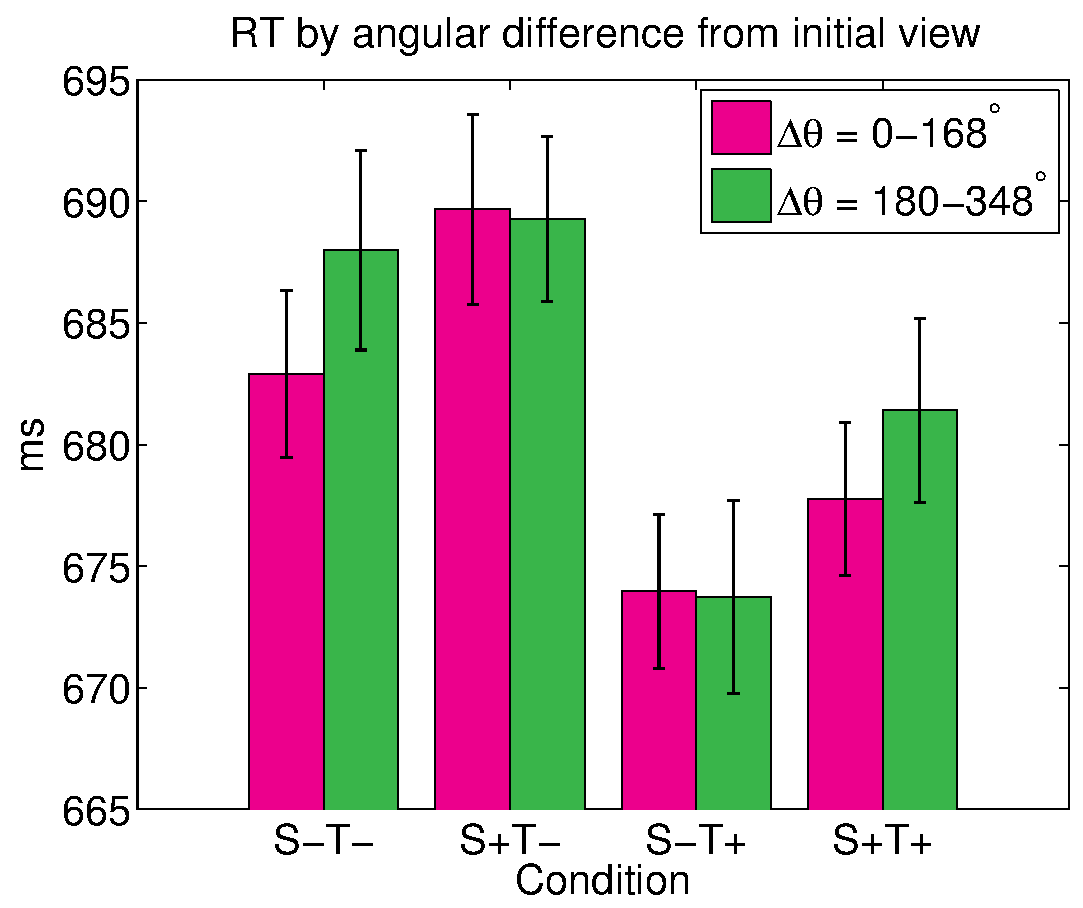
\includegraphics[width=80mm]{figs/pleast/results_rt_angle.pdf} & 
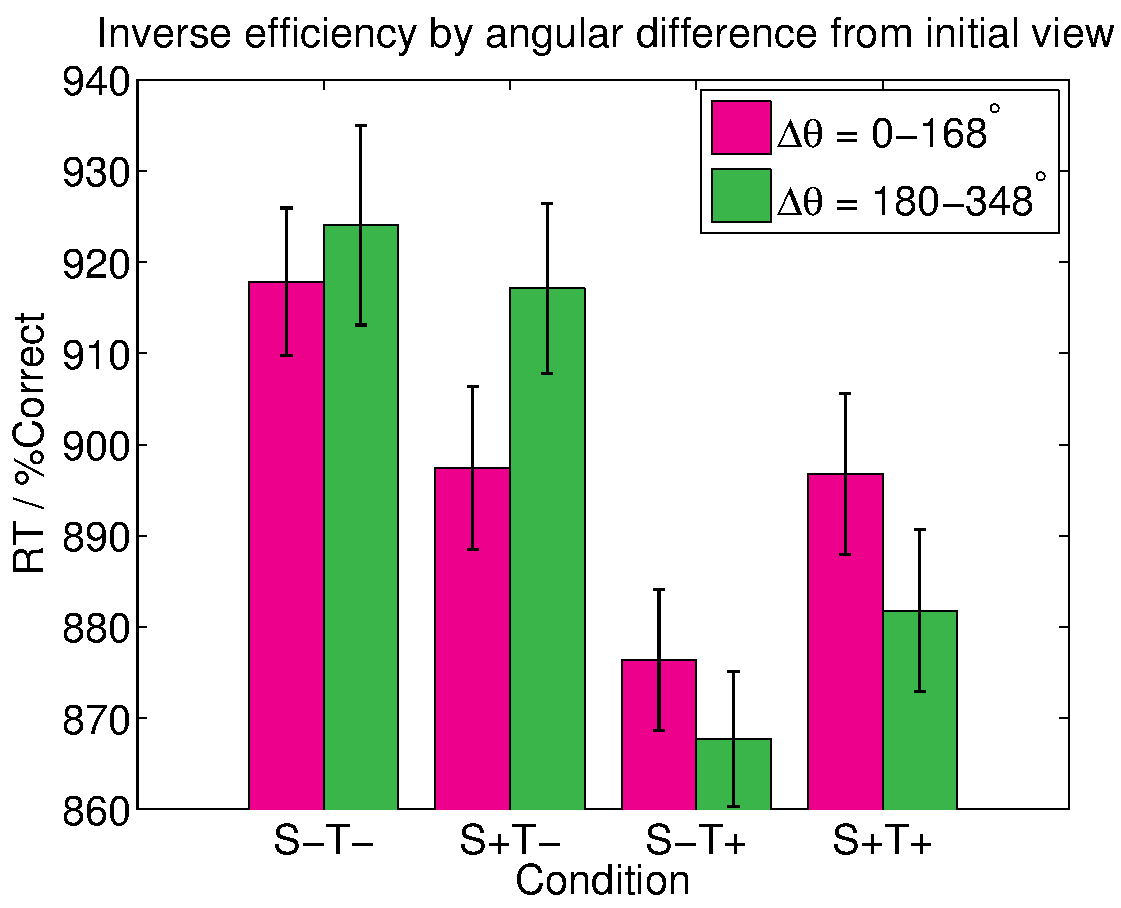
\includegraphics[width=80mm]{figs/pleast/results_ie_angle.pdf} \\
\end{tabular}
\caption{Behavioral measures for view interpolation versus extrapolation.}{}
\label{fig:behave}
\end{figure}

% on the "duh" factor of entraining at 10 Hz causes more alpha power.
% from CalderoneLakatosButlerEtAl14
% The periodicity of this effect correlated with individual resting alpha-oscillation frequency, suggesting that rhythmic stimulation recruited intrinsic oscillations rather than creating oscillations de novo. 

% just do post-hoc t-tests for angle guys -- check for effect of temporal

\bibliographystyle{apa}
\bibliography{ccnlab}
\end{document}